% !TEX root = ../ComputationalOTFnT.tex

\chapter{Extensions of Optimal Transport}
\label{c-extensions}

This chapter details several variational problems that are related to (and share the same structure of) the Kantorovich formulation of optimal transport. The goal is to extend optimal transport to more general settings: several input histograms and measures, unnormalized ones, more general classes of measures, and optimal transport between measures that focuses on local regularities (points nearby in the source measure should be mapped onto points nearby in the target measure) rather than a total transport cost, including cases where these two measures live in different metric spaces.

%%%%%%%%%%%%%%%%%%%%%%%%%%%%%%%%%%%%%%%%%%%%%%%%%%%%%%%%%%%%%%%%%%%%%%%%%%
%%%%%%%%%%%%%%%%%%%%%%%%%%%%%%%%%%%%%%%%%%%%%%%%%%%%%%%%%%%%%%%%%%%%%%%%%%
%%%%%%%%%%%%%%%%%%%%%%%%%%%%%%%%%%%%%%%%%%%%%%%%%%%%%%%%%%%%%%%%%%%%%%%%%%
\section{Multimarginal Problems}
\label{sec-multimarginal}

Instead of coupling two input histograms using the Kantorovich formulation~\eqref{eq-mk-discr}, one can couple $S$ histograms $(\a_s)_{s=1}^S$, where $\a_s \in \simplex_{n_s}$, by solving the following multimarginal problem:
\eql{\label{eq-multimarginal-discr}
	\umin{\P \in \CouplingsD(\a_s)_s}
		\dotp{\C}{\P} \eqdef \sum_s \sum_{i_s=1}^{n_s} \C_{i_1,\ldots,i_S} \P_{i_1,\ldots,i_S},
}
where the set of valid couplings is
\eq{
	\CouplingsD(\a_s)_s = \enscond{\P \in \RR^{n_1 \times \ldots \times n_S}}{
		\foralls s, \foralls i_s, \sum_{\ell \neq s} \sum_{i_\ell=1}^{n_\ell}  \P_{i_1,\ldots,i_S} = \a_{s,i_s}
	}.
} 
The entropic regularization scheme~\eqref{eq-regularized-discr} naturally extends to this setting
\eq{
	\umin{\P \in \CouplingsD(\a_s)_s}
		\dotp{\P}{\C} - \varepsilon \HD(\P), 
}
and one can then apply Sinkhorn's algorithm to compute the optimal $\P$ in scaling form, where each entry indexed by a multi-index vector $i=(i_1,\ldots,i_S)$
\eq{	
		\P_i = \K_i \prod_{s=1}^S \uD_{s,i_s}
		\qwhereq
		\K \eqdef e^{-\frac{\C}{\varepsilon}}, 
}
where $\uD_s \in \RR_+^{n_s}$ are (unknown) scaling vectors, which are iteratively updated, by cycling repeatedly through $s=1,\ldots,S$, 
\eql{\label{eq-sinkh-multimarg}
	\uD_{s,i_s} \leftarrow 
	\frac{ \a_{s,i_s} }{
		\sum_{\ell \neq s} \sum_{i_\ell=1}^{n_\ell}  \K_i \prod_{r \neq s} \uD_{\ell,i_r}
	}
}.

%%%%%%%%%%%%%%%%%%%%%
\begin{rem2}{General measures}
The discrete multimarginal problem~\eqref{eq-multimarginal-discr} is generalized to measures $(\al_s)_s$ on spaces $(\X_1,\ldots,\X_S)$ by computing a coupling measure 
\eql{\label{eq-multi-marginal-generic}
	\umin{\pi \in \Couplings(\al_s)_s} \int_{\X_1 \times \ldots \times \X_S} c(x_1,\ldots,x_S) \d\pi(x_1,\ldots,x_S),
}
where the set of couplings is 
\eq{
	\Couplings(\al_s)_s \eqdef \enscond{ \pi \in \Mm_+^1(\X_1 \times \ldots \times \X_S) }{
		\foralls s=1,\ldots,S, P_{s,\sharp} \pi = \al_s,
	}
}
where $P_s : \X_1 \times \ldots \times \X_S \rightarrow \X_s$ is the projection on the $s$th component, $P_s(x_1,\ldots,x_S)=x_s$; see, for instance,~\citep{GangboSciech}.
%
We refer to~\citep{PassMultiReview,PassMultiMarginalStructure} for a review of the main properties of the multimarginal OT problem. 
%
A typical application of multimarginal OT is to compute approximation of solutions to quantum chemistry problems, and in particular, in density functional theory~\citep{CotarDFT,GorSeiVig,BuDePGor}. This problem is obtained when considering the singular Coulomb interaction cost
\eq{
	c(x_1,\ldots,x_S) = \sum_{i \neq j} \frac{1}{\norm{x_i-x_j}}. 
}
\end{rem2}
%%%%%%%%%%%%%%%%%%%%%



%%%%%%%%%%%%%%%%%%%%%
\begin{rem2}{Multimarginal formulation of the barycenter}\label{eq-multimarg-bary}
	It is pos\-si\-ble to recast the linear program optimization~\eqref{eq-barycenter-generic} as an optimization over a single coupling over $\X^{S+1}$ where the last marginal is the barycenter and the other ones are the input measure $(\al_s)_{s=1}^S$
	\eql{\label{eq-bary-multi-full}
		\umin{ \bar \pi \in \Mm_+^1(X^{S+1}) } 
			\int_{\X^{S+1}} \sum_{s=1}^S \la_s c(x,x_s) \d\bar\pi(x_1,\ldots,x_s,x)
	}
	\eq{
		\text{subject to} \quad
				\foralls s=1,\ldots,S, \quad P_{s,\sharp}\bar\pi=\al_s.
	}
	This stems from the ``gluing lemma,'' which states that given couplings $(\pi_s)_{s=1}^S$ where $\pi_s \in \Couplings(\al_s,\al)$, one can construct a higher-dimensional coupling $\bar \pi \in \Mm_+^1(X^{S+1})$ with marginals $\pi_s$, \ie such that $Q_{s\sharp}\bar\pi=\pi_s$, where $Q_s(x_1,\ldots,x_S,x) \eqdef (x_s,x) \in \X^2$.
	\todoK{also relate this to celebrated result in graphical model, see book of Wainright/Jordan}
	% 
	By explicitly minimizing in~\eqref{eq-bary-multi-full} with respect to the last marginal (associated to $x \in \X$), one obtains that solutions $\al$ of the barycenter problem~\eqref{eq-barycenter-generic} can be computed as $\al = A_{\la,\sharp} \pi$, where $A_\la$ is the ``barycentric map'' defined as
	\eq{
		A_\la : (x_1,\ldots,x_S) \in \X^S \mapsto 
		\uargmin{x \in \X} \sum_s \la_s c(x,x_s)
	}
	(assuming this map is single-valued), where $\pi$ is any solution of the multimarginal problem~\eqref{eq-multi-marginal-generic} with cost
	\eql{\label{eq-cost-bary-multi}
		c(x_1,\ldots,x_S) = \sum_\ell \la_\ell c(x_\ell, A_\la(x_1,\ldots,x_S)).
	}
	For instance, for $c(x,y)=\norm{x-y}^2$, one has, removing the constant squared terms, 
	\eq{
		c(x_1,\ldots,x_S) = -\sum_{r \leq s} \la_r \la_s \dotp{x_r}{x_s},
	} 
	which is a problem studied in~\citet{GangboSciech}.
	%
	We refer to~\citet{Carlier_wasserstein_barycenter} for more details.
	%
	This formula shows that if all the input measures are discrete $\be_s = \sum_{i_s=1}^{n_s} \a_{s,i_s} \de_{x_{s,i_s}}$, 
	then the barycenter $\al$ is also discrete and is obtained using the formula
	\eq{
		\al = \sum_{(i_1,\ldots,i_S)} \P_{(i_1,\ldots,i_S)}
			\de_{ A_\la(x_{i_1},\ldots,x_{i_S}) }, 
	}
	where $\P$ is an optimal solution of~\eqref{eq-multimarginal-discr} with cost matrix $\C_{i_1,\ldots,i_S} = c(x_{i_1},\ldots,x_{i_S})$
	as defined in~\eqref{eq-cost-bary-multi}. Since $\P$ is a nonnegative tensor of $\prod_s n_s$ dimensions obtained as the solution of a linear program with $\sum_s n_s-S+1$ equality constraints, an optimal solution $\P$ with up to $\sum_s n_s-S+1$ nonzero values can be obtained. A barycenter $\al$ with a support of up to $\sum_s n_s-S+1$ points can therefore be obtained. This result and other considerations in the discrete case can be found in~\citet{anderes2016discrete}.
\end{rem2}
%%%%%%%%%%%%%%%%%%%%%

%%%%%%%%%%%%
\begin{rem2}{Relaxation of Euler equations}
A convex relaxation of Euler equations of incompressible fluid dynamics has been proposed by~\citeauthor{BrenierGeneralized} (\citeyear{BrenierEulerAMS}, \citeyear{BrenierEulerARMA}, \citeyear{BrenierEulerCPAM}, \citeyear{BrenierGeneralized}) and \citep{AmbrosioFigalliEuler}.
%
Similarly to the setting exposed in~\S\ref{sec-entropic-dynamic}, it corresponds to the problem of finding a probability distribution $\bar\pi \in \Mm_+^1(\bar\Xx)$ over the set $\bar\Xx$ of all paths $\ga : [0,1] \rightarrow \Xx$, which describes the movement of particules in the fluid.
%
This is a relaxed version of the initial partial differential equation model because, as in the Kantorovich formulation of OT, mass can be split. The evolution with time does not necessarily define a diffemorphism of the underlying space $\X$. 
%
The dynamic of the fluid is obtained by minimizing as in~\eqref{eq-ot-pathsspace} the energy $\int_0^1 \norm{\ga'(t)}^2 \d t$ of each path. 
%
The difference with OT over the space of paths is the additional incompressibilty of the fluid.
This incompressibilty is taken care of by imposing that the density of particules should be uniform at any time $t \in [0,1]$ (and not just imposed at initial and final times $t \in \{0,1\}$ as in classical OT). Assuming $\X$ is compact and denoting $\rho_{\Xx}$ the uniform distribution on $\Xx$, this reads $\bar P_{t,\sharp} \bar\pi = \rho_{\Xx}$ where $\bar P_t : \ga \in \bar\X \rightarrow \ga(t) \in \X$.
%
One can discretize this problem by replacing a continuous path $(\ga(t))_{t \in [0,1]}$ by a sequence of $S$ points $(x_{i_1}, x_{i_2},\ldots,x_{i_S})$ on a grid $(x_k)_{k=1}^n \subset \X$, and $\bar\Pi$ is represented by an $S$-way coupling $\P \in \RR^{n^S} \in \Couplings(\a_s)_s$, where the marginals are uniform $\a_s=n^{-1} \ones_n$. 
%
The cost of the corresponding multimarginal problem is then
\eql{\label{eq-separable-euler}
	\C_{i_1,\ldots,i_S} = \sum_{s=1}^{S-1} \norm{x_{i_s}-x_{i_{s+1}}}^2 + R \norm{x_{\sigma(i_1)}-x_{i_{S}}}^2.
}
Here $R$ is a large enough penalization constant, which is here to enforce the movement of particules between initial and final times, which is prescribed by a permutation $\sigma : \range{n} \rightarrow \range{n}$.
%
This resulting multimarginal problem is implemented efficiently in conjunction with Sinkhorn iterations~\eqref{eq-sinkh-multimarg} using the special structure of the cost, as detailed in~\citep{2015-benamou-cisc}.
%
Indeed, in place of the $O(n^S)$ cost required to compute the denominator appearing in~\eqref{eq-sinkh-multimarg}, one can decompose it as a succession of $S$ matrix-vector multiplications, hence with a low cost $Sn^2$.
%
Note that other solvers have been proposed, for instance, using the semidiscrete framework shown in~\S\ref{s-semidiscrete}; see~\citep{deGoes2015,gallouet2017lagrangian}.
\end{rem2}
%%%%%%%%%%%%


%%%%%%%%%%%%%%%%%%%%%%%%%%%%%%%%%%%%%%%%%%%%%%%%%%%%%%%%%%%%%%%%%%%%%%%%%%
%%%%%%%%%%%%%%%%%%%%%%%%%%%%%%%%%%%%%%%%%%%%%%%%%%%%%%%%%%%%%%%%%%%%%%%%%%
%%%%%%%%%%%%%%%%%%%%%%%%%%%%%%%%%%%%%%%%%%%%%%%%%%%%%%%%%%%%%%%%%%%%%%%%%%
\section{Unbalanced Optimal Transport}
\label{sec-unbalanced}

A major bottleneck of optimal transport in its usual form is that it requires the two input measures $(\al,\be)$ to have the same total mass. While many workarounds have been proposed (including renormalizing the input measure, or using dual norms such as detailed in \S~\ref{sec-dual-norms}), it is only recently that satisfying unifying theories have been developed. We only sketch here a simple but important particular case. 

Following~\citet{LieroMielkeSavareLong}, to account for arbitrary positive histograms $(\a,\b) \in \RR_+^n \times \RR_+^m$, the initial Kantorovich formulation~\eqref{eq-mk-discr} is ``relaxed'' by only penalizing marginal deviation using some divergence $\DivergmD_\phi$, defined in~\eqref{eq-discr-diverg}. This equivalently corresponds to minimizing an OT distance between approximate measures
\begin{align}\label{eq-unbalanced-pbm}
	\MKD_{\C}^\tau(\a,\b) &= \umin{\tilde\a,\tilde\b} \MKD_{\C}(\a,\b) + \tau_1 \DivergmD_\phi(\a,\tilde \a) + \tau_2 \DivergmD_\phi(\b,\tilde\b) \\
		&= \umin{\P \in \RR_+^{n \times m}} \dotp{\C}{\P} + \tau_1\DivergmD_\phi(\P\ones_m|\a) + \tau_2\DivergmD_\phi(\P^\top\ones_m|\b), 
\end{align}
where $(\tau_1,\tau_2)$ controls how much mass variations are penalized as opposed to transportation of the mass. In the limit $\tau_1=\tau_2 \rightarrow +\infty$, assuming $\sum_i \a_i=\sum_j \b_j$ (the ``balanced'' case), one recovers the original optimal transport formulation with hard marginal constraint~\eqref{eq-mk-discr}. 

This formalism recovers many different previous works, for instance introducing for $\DivergmD_\phi$ an $\ell^2$ norm~\citep{benamou2003numerical} or an $\ell^1$ norm as in partial transport~\citep{FigalliPartial,CaffarelliMcCannPartial}. 
%
A case of particular importance is when using $\DivergmD_\phi=\KLD$ the Kulback--Leibler divergence, as detailed in Remark~\ref{rem-wfr-static}.
%
For this cost, in the limit $\tau=\tau_1=\tau_2 \rightarrow 0$, one obtains the so-called squared Hellinger distance (see also Example~\ref{exmp-hellinger})
\eq{
	\MKD_{\C}^\tau(\a,\b) \overset{\tau \rightarrow 0}{\longrightarrow}
	\Hellinger^2(\a,\b) = \sum_i ( \sqrt{\a_i}-\sqrt{\b_i} )^2.
}

Sinkhorn's iterations~\eqref{eq-sinkhorn} can be adapted to this problem by making use of the generalized algorithm detailed in~\S\ref{sec-generalized}. The solution has the form~\eqref{eq-scaling-form} and the scalings are updated as
\eql{\label{eq-iterate-gen-sinkh}
	\uD \leftarrow \pa{ \frac{\a}{\K \vD} }^{\frac{\tau_1}{\tau_1+\varepsilon}}
	\qandq
	\vD \leftarrow \pa{ \frac{\b}{\transp{\K}\uD} }^{\frac{\tau_2}{\tau_2+\varepsilon}}.
}

%%%%%%%%%%%%%%%%%%%%%
\begin{rem2}{Generic measure}
For $(\al,\be)$ two arbitrary measures, the unbalanced version (also called ``log-entropic'') of~\eqref{eq-mk-generic} reads
\begin{align*}
	\MK_\c^\tau(\al,\be) \eqdef 
	&\umin{\pi \in \Mm_+(\X \times \Y)}
		\int_{\X \times \Y} \c(x,y) \d\pi(x,y) \\
		&+ \tau \Divergm_\phi(P_{1,\sharp}\pi|\al)
		+ \tau \Divergm_\phi(P_{2,\sharp}\pi|\be),
\end{align*}
where divergences $\Divergm_\phi$ between measures are defined in~\eqref{eq-phi-div}.
%
In the special case $c(x,y) = \norm{x-y}^2$, $\Divergm_\phi=\KL$, $\MK_\c^\tau(\al,\be)^{1/2}$ is the Gaussian--Hellinger distance~\citep{LieroMielkeSavareLong}, and it is shown to be a distance on $\Mm_+^1(\RR^d)$. 
\end{rem2}
%%%%%%%%%%%%%%%%%%%%%

%%%%%%%%%%%%%%%%%%%%%
\begin{rem2}{Wasserstein--Fisher--Rao}\label{rem-wfr-static}
For the particular choice of cost
\eq{
	c(x,y) = -\log \cos(\min(\dist(x,y)/\kappa,\pi/2)),
}
where $\kappa$ is some cutoff distance, and using $\Divergm_\phi=\KL$, then
\eq{
	\WFR(\al,\be) \eqdef \MK_\c^\tau(\al,\be)^{\frac{1}{2}}
} 
is the so-called Wasserstein--Fisher--Rao or Hellinger--Kantorovich distance. 
%
In the special case $\X=\RR^d$, this static (Kantorovich-like) formulation matches its dynamical counterparts~\eqref{eq-wfr-dynamic}, as proved independently by~\citet{LieroMielkeSavareLong,2015-chizat-unbalanced}. This dynamical formulation is detailed in~\S\ref{dynamic-unbalanced}.
%
%It is a distance on $\Mm_+^1(\X)$. In the special case $\X=\RR^d$, it also has a dynamic interpretation, which in some sense shows that it is the canonical extension of the $\Wass_2$ to the unbalanced case. It generalizes the initial Benamou-Brenier dynamical formulation~\eqref{eq-bb-convex} by introducing a source term $s_t(x)$ which is a scalar valued measure
%\begin{align*}
%	\WFR(\al_0,\al_1)^2 = &\umin{ (\al_t,\Moment_t,s_t)_t  \in \bar\BBConstr(\al_0,\al_1)  }
%		\int_0^1 \int_{\RR^d} \theta(\al_t(x),\Moment_t(x)) \\
%		& +  \theta(\al_t(x),s_t(x)) \d x \d t
%\end{align*}
%and the continuity equation reads
%\eq{
%	\bar\BBConstr(\al_0,\al_1) \eqdef 
%	\enscond{ (\al_t,\Moment_t,s_t) }{
%		\pd{\al_t}{t} + \diverg(\Moment_t) = s_t, 
%		\al_{t=0,1}=\al_{0,1}
%	}.
%}
%It can be solved using very similar methods to those detailed in Chapter~\ref{c-dynamic}. 
\end{rem2}
%%%%%%%%%%%%%%%%%%%%%

The barycenter problem~\eqref{eq-barycenter-generic} can be generalized to handle an unbalanced setting by replacing $\MK_{\c}$ with $\MK_\c^\tau$. 
%
Figure~\ref{fig-interpolation-static} shows the resulting interpolation, providing a good illustration of the usefulness of the relaxation parameter $\tau$. 
%
The input measures are mixtures of two Gaussians with unequal mass. Classical OT requires the leftmost bump to be split in two and gives a nonregular interpolation. In sharp contrast, unbalanced OT allows the mass to vary during interpolation, so that the bumps are not split and local modes of the distributions are smoothly matched.
%
Using finite values for $\tau$ (recall that OT is equivalent to $\tau=\infty)$ is thus important to prevent irregular interpolations that arise because of mass splitting, which happens because of a ``hard'' mass conservation constraint.
%
The resulting optimization problem can be tackled numerically using entropic regularization and the generalized Sinkhorn algorithm detailed in~\S\ref{sec-generalized}. 

In practice, unbalanced OT techniques seem to outperform classical OT for applications (such as in imaging or machine learning) where the input data is noisy or not perfectly known. They are also crucial when the signal strength of a measure, as measured by its total mass, must be accounted for, or when normalization is not meaningful. This was the original motivation of~\citet{FrognerNIPS}, whose goal was to compare sets of word labels used to describe images. Unbalanced OT and the corresponding Sinkhorn iterations have also been used for applications to the dynamics of cells in~\citep{schiebinger2017reconstruction}.

\begin{figure}[h!]
\centering
\begin{tabular}{@{}c@{\hspace{10mm}}c@{}}
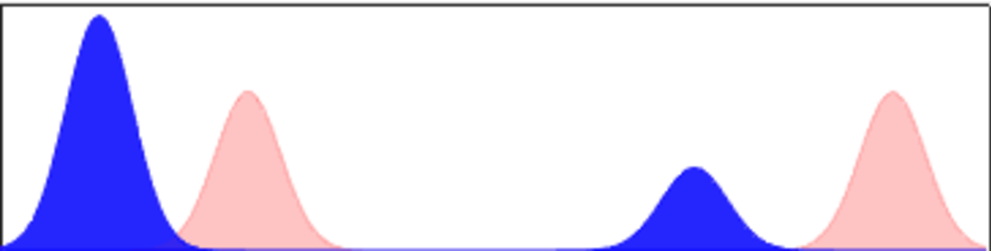
\includegraphics[width=.4\linewidth]{unbalanced/ot-1} & 
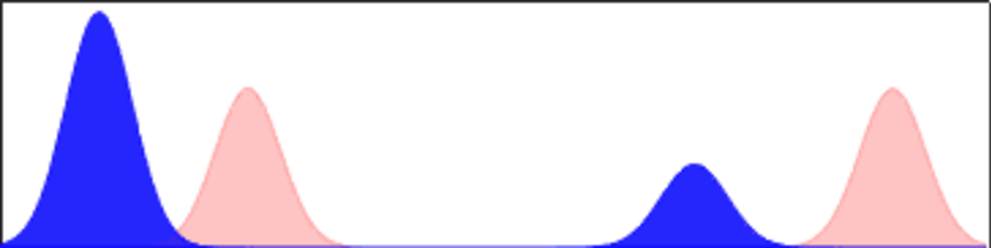
\includegraphics[width=.4\linewidth]{unbalanced/unbal-1} \\
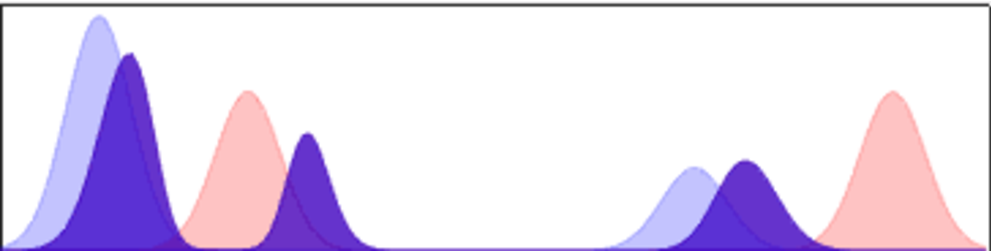
\includegraphics[width=.4\linewidth]{unbalanced/ot-2} & 
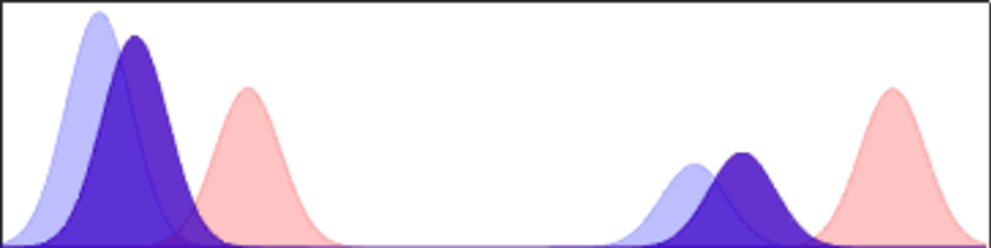
\includegraphics[width=.4\linewidth]{unbalanced/unbal-2} \\
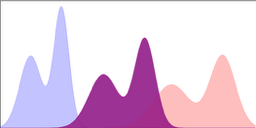
\includegraphics[width=.4\linewidth]{unbalanced/ot-3} & 
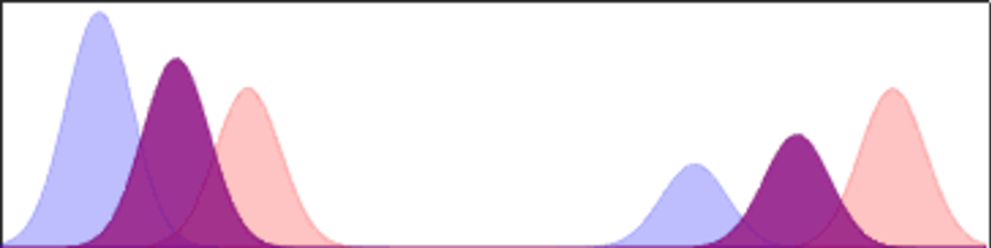
\includegraphics[width=.4\linewidth]{unbalanced/unbal-3} \\
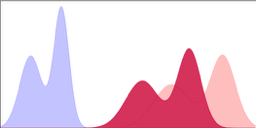
\includegraphics[width=.4\linewidth]{unbalanced/ot-4} & 
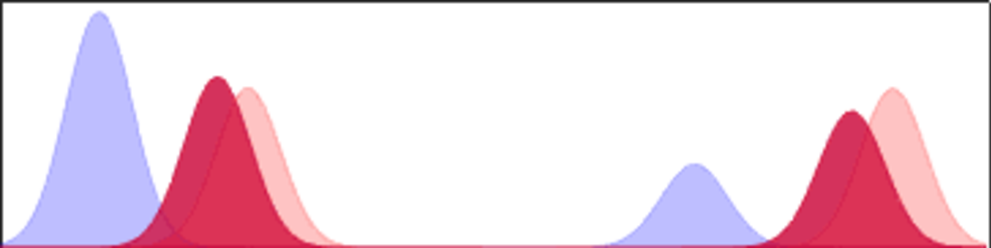
\includegraphics[width=.4\linewidth]{unbalanced/unbal-4} \\
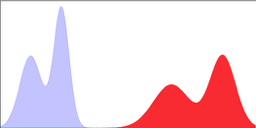
\includegraphics[width=.4\linewidth]{unbalanced/ot-5} & 
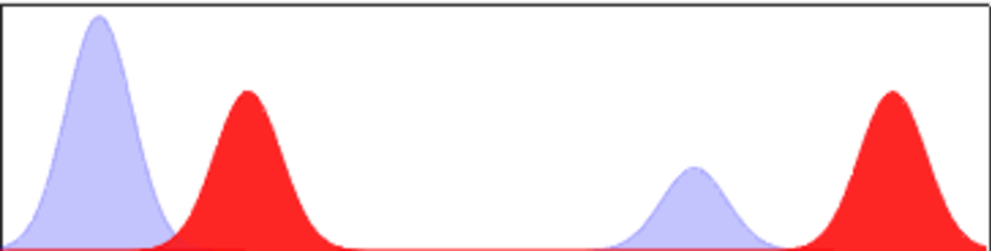
\includegraphics[width=.4\linewidth]{unbalanced/unbal-5} \\
Classical OT ($\tau=+\infty$) & Ubalanced OT ($\tau=1$)
\end{tabular}
%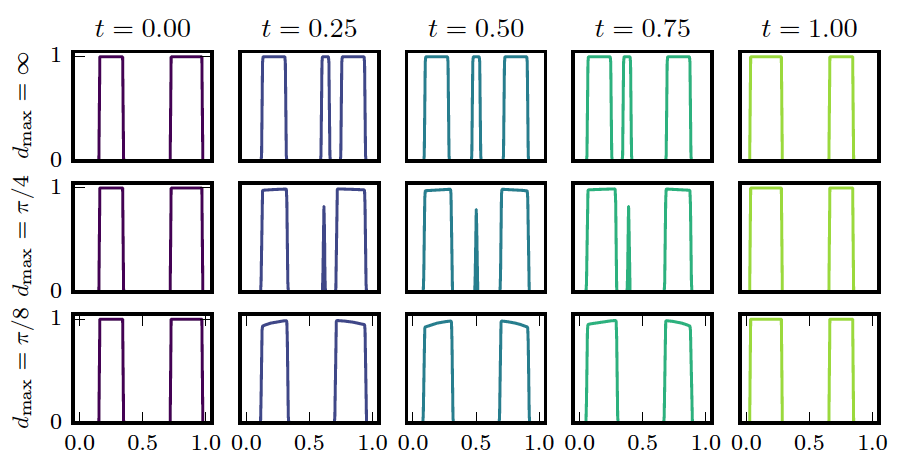
\includegraphics[width=\linewidth]{unbalanced/interpolation-static}
\caption{\label{fig-interpolation-static}
Influence of relaxation parameter $\tau$ on unbalanced barycenters.
Top to bottom: the evolution of the barycenter between two input measures.
}
\end{figure}


%%%
\begin{rem}[Connection with dual norms]\label{rem-unb-dualnorms}
A particularly simple setup to account for mass variation is to use dual norms, as detailed in~\S\ref{sec-dual-norms}. By choosing a compact set $B \subset \Cc(\X)$ one obtains a norm defined on the whole space $\Mm(\X)$ (in particular, the measures do not need to be positive). A particular instance of this setting is the flat norm~\eqref{eq-set-flatnorm}, which is recovered as a special instance of unbalanced transport, when using $\Divergm_\phi(\al|\al')=\norm{\al-\al'}_{\TV}$ to be the total variation norm~\eqref{eq-defn-tv}; see, for instance,~\citep{hanin1992kantorovich,lellmann2014imaging}. 
%
We also refer to~\citep{schmitzer2017framework} for a general framework to define Wasserstein-1 unbalanced transport.
\end{rem}
%%%%

%%%%%%%%%%%%%%%%%%%%%%%%%%%%%%%%%%%%%%%%%%%%%%%%%%%%%%%%%%%%%%%%%%%%%%%%%%
%%%%%%%%%%%%%%%%%%%%%%%%%%%%%%%%%%%%%%%%%%%%%%%%%%%%%%%%%%%%%%%%%%%%%%%%%%
%%%%%%%%%%%%%%%%%%%%%%%%%%%%%%%%%%%%%%%%%%%%%%%%%%%%%%%%%%%%%%%%%%%%%%%%%%
\section{Problems with Extra Constraints on the Couplings}

Many other OT-like problems have been proposed in the literature. They typically correspond to adding extra constraints $\Cc$ on the set of feasible couplings appearing in the original OT problem~\eqref{eq-mk-generic}
\eql{\label{ot-extra-constr}
	\umin{\pi \in \Couplings(\al,\be)}
		\enscond{ \int_{\X \times \Y} \c(x,y) \d\pi(x,y) }{ \pi \in \Cc }.
}	
Let us give two representative examples.
%
The optimal transport with capacity constraint~\citep{km1} corresponds to imposing that the density $\density{\pi}$ (for instance, with respect to the Lebesgue measure) is upper bounded
\eql{\label{eq-capacity-constr}
	\Cc = \enscond{ \pi }{ \density{\pi} \leq \kappa }
}
for some $\kappa>0$. This constraint rules out singular couplings localized on Monge maps. 
%
The martingale transport problem (see, for instance,~\citet{GalichonMartingale,dolinsky2014martingale,TanTouzi,beiglbock2013model}), which finds many applications in finance, imposes the so-called martingale constraint on the conditional mean of the coupling, when $\X=\Y=\RR^d$:
\eql{\label{eq-martingale-constr}
	\Cc = \enscond{ \pi }{ \foralls x \in \RR^d,  \int_{\RR^d} y \frac{\d \pi(x,y)}{\d\al(x)\d\be(y)} \d\be(y) = x }.
}
This constraint imposes that the barycentric projection map~\eqref{eq-bary-proj} of any admissible coupling must be equal to the identity.
%
For arbitrary $(\al,\be)$, this set $\Cc$ is typically empty, but necessary and sufficient conditions exist ($\al$ and $\be$ should be in ``convex order'') to ensure $\Cc \neq \emptyset$ so that  $(\al,\be)$ satisfy a martingale constraint. This constraint can be difficult to enforce numerically when discretizing an existing problem.
%
It also forbids the solution to concentrate on a single Monge map, and can lead to couplings concentrated on the union of several graphs (a ``multivalued'' Monge map), or even more complicated support sets.
%
Using an entropic penalization as in~\eqref{eq-entropic-generic}, one can solve approximately~\eqref{ot-extra-constr} using the Dykstra algorithm as explained in~\citet{2015-benamou-cisc}, which is a generalization of Sinkhorn's algorithm shown in~\S\ref{sec-sinkhorn}. This requires computing the projection onto $\Cc$ for the $\KL$ divergence, which is straightforward for~\eqref{eq-capacity-constr} but cannot be done in closed form~\eqref{eq-martingale-constr} and thus necessitates subiterations; see~\citep{guo2017computational} for more details.


%%%%%%%%%%%%%%%%%%%%%%%%%%%%%%%%%%%%%%%%%%%%%%%%%%%%%%%%%%%%%%%%%%%%%%%%%%
%%%%%%%%%%%%%%%%%%%%%%%%%%%%%%%%%%%%%%%%%%%%%%%%%%%%%%%%%%%%%%%%%%%%%%%%%%
%%%%%%%%%%%%%%%%%%%%%%%%%%%%%%%%%%%%%%%%%%%%%%%%%%%%%%%%%%%%%%%%%%%%%%%%%%
\section{Sliced Wasserstein Distance and Barycenters}\label{sec-sliced}

One can define a distance between two measures $(\al,\be)$ defined on $\RR^\dim$ by aggregating 1-D Wasserstein distances between their projections onto all directions of the sphere. This defines
\eql{\label{eq-sw-def}
	\SW(\al,\be)^2 \eqdef \int_{\SS^d} \Wass_2( P_{\th,\sharp} \al, P_{\th,\sharp} \be )^2 \d\th,
}
where $\SS^\dim = \ensconds{\th \in \RR^\dim}{\norm{\th}=1}$ is the $\dim$-dimensional sphere, and $P_\th : x \in \RR^\dim \rightarrow \RR$ is the projection. This approach is detailed in~\citep{2013-Bonneel-barycenter}, following ideas from Marc Bernot. It is related to the problem of Radon inversion over measure spaces~\citep{AbrahamRadon}. 

%%%
\paragraph{Lagrangian discretization and stochastic gradient descent. }

The advantage of this functional is that 1-D Wasserstein distances are simple to compute, as detailed in~\S\ref{sec:specialcases}. In the specific case where $m=n$ and 
\eql{\label{eq-lagrangian-sliced}
	\al=\frac{1}{n}\sum_{i=1}^n \de_{x_i}
	\qandq 
	\be=\frac{1}{n}\sum_{i=1}^m \de_{y_i}, 
}
this is achieved by simply sorting points
\eq{
	\SW(\al,\be)^2 = \int_{\SS^d} \pa{
		 \sum_{i=1}^n | \dotp{ x_{\si_\th(i)} - y_{\kappa_\th(i)} }{\th} |^2 
		}
		\d\th,
}
where $\si_\th,\kappa_\th \in \Perm(n)$ are the permutation ordering in increasing order, respectively, $(\dotp{x_i}{\th})_i$ and $(\dotp{y_i}{\th})_i$. 

Fixing the vector $y$, the function $\Ee_\be(x) \eqdef \SW(\al,\be)^2$ is smooth, and one can use this function to define a mapping by gradient descent 
\eql{\label{eq-grad-sliced-lagr}
	x \leftarrow x - \tau \nabla\Ee_\be(x)
	\qwhereq
}
\eq{
	\nabla\Ee_\be(x)_i = 
		2 \int_{\SS^d} \pa{
		 	\dotp{ x_{i} - y_{\kappa_\th \circ \si_\th^{-1}(i)} }{\th}  \th
		}
		\d\th
}
using a small enough step size $\tau>0$. 
%
To make the method tractable, one can use a stochastic gradient descent (SGD), replacing this integral with a discrete sum against randomly drawn directions $\th \in \SS^\dim$ (see~\S\ref{sec-sgd} for more details on SGD). 
%
The flow~\eqref{eq-grad-sliced-lagr} can be understood as (Langrangian implementation of) a Wasserstein gradient flow (in the sense of~\S\ref{sec-grad-flows}) of the function $\al \mapsto \SW(\al,\be)^2$. Numerically, one finds that this flow has no local minimizer and that it thus converges to $\al=\be$. The usefulness of the Lagrangian solver is that, at convergence, it defines a matching (similar to a Monge map) between the two distributions. This method has been used successfully for color transfer and texture synthesis in~\citep{rabin-ssvm-11} and is related to the alternate minimization approach detailed in~\citep{pitie2007automated}.

It is simple to extend this Lagrangian scheme to compute approximate ``sliced'' barycenters  of measures, by mimicking the Frechet definition of Wasserstein barycenters~\eqref{eq-barycenter-generic} and minimizing 
\eql{\label{eq-barycenter-sliced}
		\umin{\al \in \Mm_+^1(\X)} \sum_{s=1}^S \la_s \SW(\al,\be_s)^2,
}
given a set $(\be_s)_{s=1}^S$ of fixed input measure. Using a Lagrangian discretization of the form~\eqref{eq-lagrangian-sliced} for both $\al$ and the $(\be_s)_s$, one can perform the nonconvex minimization over the position $x=(x_i)_i$
\eql{\label{eq-bary-lagrangian-sliced}
	\umin{x} \Ee(x) \eqdef \sum_{s} \la_s \Ee_{\be_s}(x),
	\qandq 
	\nabla \Ee(x) = \sum_{s} \la_s \nabla \Ee_{\be_s}(x), 
}
by gradient descent using formula~\eqref{eq-grad-sliced-lagr} to compute $\nabla \Ee_{\be_s}(x)$ (coupled with a random sampling of the direction $\th$).




%%%
\paragraph{Eulerian discretization and Radon transform. }

A related way to compute an approximated sliced barycenter, without resorting to an iterative minimization scheme, is to use the fact that~\eqref{eq-sw-def} computes a distance between the Radon transforms $\Rr(\al)$ and $\Rr(\be)$ where
\eq{
	\Rr(\al) \eqdef ( P_{\th,\sharp} \al )_{\th \in \SS^d}.
}
A crucial point is that the Radon transform is invertible and that its inverse can be computed using a filtered backprojection formula. 
%
Given a collection of measures $\rho = (\rho_\th)_{\th \in \SS^d}$, one defines the filtered  backprojection operator as
\eql{\label{eq-filter-backproj}
	\Rr^+(\rho) = C_\dim \De^{\frac{d-1}{2}} \Bb(\rho),
}
where $\xi = \Bb(\rho) \in \Mm(\RR^d)$ is the measure defined through the relation 
\eql{\label{eq-backproj}
	\foralls g \in \Cc(\RR^d), \quad
	\int_{\RR^d} g(x) \d\xi(x) = 
	\int_{\SS^d}  \int_{\RR^{\dim-1}}   \int_{\RR}   
		g( r \th + U_\th z ) 
	\d \rho_\th(r) \d z \d \th,
}
where $U_\th$ is any orthogonal basis of $\th^\bot$, 
and where $C_\dim \in \RR$ is a normalizing constant which depends on the dimension.
%
Here $\De^{\frac{d-1}{2}}$ is a fractional Laplacian, which is the high-pass filter defined over the Fourier domain as 
$\hat \De^{\frac{d-1}{2}}(\om) = \norm{\om}^{d-1}$.
%
The definition of the backprojection~\eqref{eq-backproj} adds up the contribution of all the measures $(\rho_\th)_\th$ by extending each one as being constant in the directions orthogonal to $\th$.
%
One then has the left-inverse relation $\Rr^+ \circ \Rr = \Identity_{\Mm(\RR^\dim)}$, so that $\Rr^+$ is a valid reconstruction formula. 


\newcommand{\MyFigRadon}[1]{\includegraphics[width=.19\linewidth]{radon-bary/#1}}
\begin{figure}[h!]
\centering
\begin{tabular}{@{}c@{\hspace{1mm}}c@{\hspace{1mm}}c@{\hspace{1mm}}c@{\hspace{1mm}}c@{}}
\MyFigRadon{bary-1} &
\MyFigRadon{bary-3} &
\MyFigRadon{bary-5} &
\MyFigRadon{bary-7} &
\MyFigRadon{bary-9} \\
\MyFigRadon{radon-1} &
\MyFigRadon{radon-3} &
\MyFigRadon{radon-5} &
\MyFigRadon{radon-7} &
\MyFigRadon{radon-9} \\
$t=0$ & $t=1/4$ & $t=1/2$ & $t=3/4$ & $t=1$  
\end{tabular}
\caption{\label{fig-radon-bary}
Example of sliced barycenters computation using the Radon transform (as defined in~\eqref{eq-barycenter-radon-sliced}). 
%
Top: barycenters $\al_t$ for $S=2$ two input and weights $(\la_1,\la_2)=(1-t,t)$. 
Bottom: their Radon transform $\Rr(\al_t)$ (the horizontal axis being the orientation angle $\th$). 
}
\end{figure}

In order to compute barycenters of input densities, it makes sense to replace formula~\eqref{eq-barycenter-generic} by its equivalent using Radon transform, and thus consider independently for each $\th$ the 1-D barycenter problem
\eql{\label{eq-barycenter-radon-sliced}
		\rho_\th^\star \in \uargmin{ (\rho_\th \in \Mm_+^1(\RR)) } \sum_{s=1}^S \la_s \Wass_2( \rho_\th, P_{\th,\sharp} \be_s)^2.
}
Each 1-D barycenter problem is easily computed using the monotone rearrangement as detailed in Remark~\ref{rem-bary-1d}.
%
The Radon approximation $\al_{R} \eqdef \Rr^+( \rho^\star )$ of a sliced barycenter solving~\eqref{eq-barycenter-generic} is then obtained by the inverse Radon transform $\Rr^+$. Note that in general, $\al_R$ is not a solution to~\eqref{eq-barycenter-generic} because the Radon transform is not surjective, so that  $\rho^\star$, which is obtained as a barycenter of the Radon transforms $\Rr(\be_s)$ does not necessarily belong to the range of $\Rr$. But numerically it seems in practice to be almost the case~\citep{2013-Bonneel-barycenter}.
%
Numerically, this Radon transform formulation is very effective for input measures and barycenters discretized on a fixed grid (\emph{e.g.} a uniform grid for images), and $\Rr$ and well as $\Rr^+$ are computed approximately on this grid using fast algorithms (see, for instance,~\citep{FastSlantStack}).
%
Figure~\ref{fig-radon-bary} illustrates this computation of barycenters (and highlights the way the Radon transforms are interpolated), while Figure~\ref{fig-sliced-bary-compar} shows a comparison of the Radon barycenters~\eqref{eq-barycenter-radon-sliced} and the ones obtained by Lagrangian discretization~\eqref{eq-bary-lagrangian-sliced}.


\begin{figure}[h!]
\centering
\begin{tabular}{@{}c@{\hspace{1mm}}c@{\hspace{1mm}}c@{}}
\includegraphics[width=.32\linewidth]{sliced/triangle-radon}&
\includegraphics[width=.32\linewidth]{sliced/triangle-sliced}&
\includegraphics[width=.32\linewidth]{sliced/triangle-wass} \\
Radon & Lagrangian & Wasserstein
\end{tabular}
\caption{\label{fig-sliced-bary-compar}
Comparison of barycenters computed using Radon transform~\eqref{eq-barycenter-radon-sliced} (Eulerian discretization), Lagrangian discretization~\eqref{eq-bary-lagrangian-sliced}, and Wasserstein OT (computed using Sinkhorn iterations~\eqref{eq-sinkhorn-bary}). 
}
\end{figure}



%%%
\paragraph{Sliced Wasserstein kernels.}

Beside its computational simplicity, another advantage of the sliced Wasserstein distance is that it is isometric to a Euclidean distance (it is thus a ``Hilbertian'' metric), as detailed in Remark~\ref{rem-1d-ot-generic}, and in particular formula~\eqref{eq-wass-cumul}. 
% 
As highlighted in~\S\ref{sec-non-embeddability}, this should be contrasted with the Wasserstein distance $\Wass_2$ on $\RR^\dim$, which is not Hilbertian in dimension $\dim \geq 2$. 
%
It is thus possible to use this sliced distance to equip the space of distributions $\Mm_1^+(\RR^\dim)$ with a reproducing kernel Hilbert space structure (as detailed in~\S\ref{sec-non-embeddability}). 
%
One can, for instance, use the exponential and energy distance kernels
\eq{
	\Krkhs(\al,\be) = e^{-\frac{\SW(\al,\be)^p}{2\si^p}}
	\qandq
	\Krkhs(\al,\be) = -\SW(\al,\be)^p
}
for $1 \leq p \leq 2$ for the exponential kernels and $0 < p < 2$ for the energy distance kernels.
%
This means that for any collection $(\al_i)_i$ of input measures, the matrix $( \Krkhs(\al_i,\al_j) )_{i,j}$ is symmetric positive semidefinite. It is possible to use these kernels to perform a variety of machine learning tasks using the ``kernel trick,'' for instance, in regression, classification (SVM and logistic), clustering (K-means) and dimensionality reduction (PCA)~\citep{Hofmann2008}.
%
We refer to~\citet{kolouri2016sliced} for details and applications.



%%%%%%%%%%%%%%%%%%%%%%%%%%%%%%%%%%%%%%%%%%%%%%%%%%%%%%%%%%%%%%%%%%%%%%%%%%
%%%%%%%%%%%%%%%%%%%%%%%%%%%%%%%%%%%%%%%%%%%%%%%%%%%%%%%%%%%%%%%%%%%%%%%%%%
%%%%%%%%%%%%%%%%%%%%%%%%%%%%%%%%%%%%%%%%%%%%%%%%%%%%%%%%%%%%%%%%%%%%%%%%%%
\section{Transporting Vectors and Matrices}

Real-valued measures $\al \in \Mm(\Xx)$ are easily generalized to vector-valued measures $\al \in \Mm(\Xx;\VV)$, where $\VV$ is some vector space. For notational simplicity, we assume $\VV$ is Euclidean and equipped with some inner product $\dotp{\cdot}{\cdot}$ (typically $\VV=\RR^\dim$ and the inner product is the canonical one). Thanks to this inner product, vector-valued measures are identified with the dual of continuous functions $g : \Xx \rightarrow \VV$, \ie for any such $g$, one defines its integration against the measure as 
\eql{\label{eq-integration-vec-valued}
	\int_\Xx g(x) \d\al(x) \in \RR,
}
which is a linear operation on $g$ and $\al$. A discrete measure has the form $\al = \sum_i \a_i \de_{x_i}$ where $(x_i,a_i) \in \Xx \times \VV$ and the integration formula~\eqref{eq-integration-vec-valued} simply reads
\eq{
	\int_\Xx g(x) \d\al(x) = \sum_i \dotp{\a_i}{g(x_i)} \in \RR.
}
Equivalently, if $\VV=\RR^\dim$, then such an $\al$ can be viewed as a collection $(\al_s)_{s=1}^\dim$ of $\dim$ ``classical'' real-valued measures (its coordinates), writing  
\eq{
	\int_\Xx g(x) \d\al(x) =  \sum_{s=1}^\dim \int_\Xx g_s(x) \d\al_s(x), 
}
where $g(x)=(g_s(x))_{s=1}^\dim$ are the coordinates of $g$ in the canonical basis. 

%%%
\paragraph{Dual norms.}

It is nontrivial, and in fact in general impossible, to extend OT distances to such a general setting. Even coping with real-valued measures taking both positive and negative values is difficult. The only simple option is to consider dual norms, as defined in~\S\ref{sec-dual-norms}. Indeed, formula~\eqref{eq-w1-cont} readily extends to $\Mm(\Xx;\VV)$ by considering $B$ to be a subset of $\Cc(\Xx;\VV)$. So in particular, $\Ww_1$, the flat norm and MMD norms can be computed for vector-valued measures. 

%%%
\paragraph{OT over cone-valued measures. }

It is possible to define more advanced OT distances when $\al$ is restricted to be in a subset $\Mm(\Xx;\Vv) \subset \Mm(\Xx;\VV)$. The set $\Vv$ should be a positively 1-homogeneous convex cone of $\VV$
\eq{
	\Vv \eqdef \enscond{ \la u }{ \la \in \RR^+,  u \in \Vv_0, }
}
where $\Vv_0$ is a compact convex set. 
%
A typical example is the set of positive measures where $\Vv=\RR_+^\dim$. Dynamical convex formulations of OT over such a cone have been proposed; see~\citep{MatthesPositive}. This has been applied to model the distribution of chemical components. 
%
Another important example is the set of positive symmetric matrices $\Vv=\Ss_+^\dim \subset \RR^{\dim \times \dim}$. It is of course possible to use dual norms over this space, by treating matrices as vectors; see, for instance,~\citep{Ning2014metrics}. Dynamical convex  formulations for OT over such a cone have been provided~\citep{Chen2016,JiangSpectral}. Some static (Kantorovich-like) formulations also have been proposed~\citep{ning2015matrix,2016-peyre-qot}, but a mathematically sound theoretical framework is still missing. In particular, it is unclear if these static approaches define distances for vector-valued measures and if they relate to some dynamical formulation.  Figure~\ref{fig-tensors} is an example of tensor interpolation obtained using the method detailed in~\citep{2016-peyre-qot}, which proposes a generalization of Sinkhorn algorithms using quantum relative entropy~\eqref{eq-quantum-entropy} to deal with tensor fields.

%%%
\paragraph{OT over positive matrices. }

A related but quite different setting is to replace discrete measures, \ie histograms $\a \in \Si_n$, by positive matrices with unit trace $A \in \Ss_n^+$ such that $\tr(A)=1$. The rationale is that the eigenvalues $\la(A) \in \Si_n$ of $A$ play the role of a histogram, but one also has to take care of the rotations of the eigenvectors, so that this problem is more complicated.

One can extend several divergences introduced in~\S\ref{sec-phi-div} to this setting. For instance, the Bures metric~\eqref{eq-bure-defn} is a generalization of the Hellinger distance (defined in Remark~\ref{exmp-hellinger}), since they are equal on positive diagonal matrices. 
%
One can also extend the Kullback--Leibler divergence~\eqref{eq-kl-defn} (see also Remark~\ref{ex_KLdiv}), which is generalized to positive matrices as
\eql{\label{eq-quantum-entropy}
	\KLD(A|B) \eqdef \tr\pa{ P \log(P)-P\log(Q)-P+Q, }
}
where $\log(\cdot)$ is the matrix logarithm. This matrix $\KLD$ is convex with both of its arguments. 

It is possible to solve convex dynamic formulations to define OT distances between such matrices~\citep{Carlen2014,Chen2016,ChenGangbo17}. There also exists an equivalent of Sinkhorn's algorithm, which is due to~\citet{gurvits2004classical} and has been extensively studied in~\citep{georgiou2015positive}; see also the review paper~\citep{ReviewSinkhorn}. It is known to converge only in some cases but seems empirically to always work.


\newcommand{\MyFigTensorMesh}[1]{\includegraphics[width=.100\linewidth,trim=140 10 120 0,clip]{tensors/mesh/interpol-#1}}
\newcommand{\MyFigTensorImg}[1]{\includegraphics[width=.105\linewidth,trim=80 20 80 20,clip]{tensors/2d/interpol-ellipses-#1}}
%%% FIG %%%
\begin{figure}[h!]\centering
\centering
\begin{tabular}{@{\hspace{1mm}}c@{\hspace{1mm}}c@{\hspace{1mm}}c@{\hspace{1mm}}c@{\hspace{1mm}}c@{\hspace{1mm}}c@{\hspace{1mm}}c@{\hspace{1mm}}c@{\hspace{1mm}}c@{}}
\MyFigTensorImg{1}&
\MyFigTensorImg{2}&
\MyFigTensorImg{3}&
\MyFigTensorImg{4}&
\MyFigTensorImg{5}&
\MyFigTensorImg{6}&
\MyFigTensorImg{7}&
\MyFigTensorImg{8}&
\MyFigTensorImg{9}\\
\MyFigTensorMesh{1}&
\MyFigTensorMesh{2}&
\MyFigTensorMesh{3}&
\MyFigTensorMesh{4}&
\MyFigTensorMesh{5}&
\MyFigTensorMesh{6}&
\MyFigTensorMesh{7}&
\MyFigTensorMesh{8}&
\MyFigTensorMesh{9}\\
$t=0$ & $t=1/8$ & $t=1/4$ & $t=3/8$ & $t=1/2$ & $t=5/8$ & $t=3/4$ & $t=7/8$ & $t=1$ 
\end{tabular}
%%%
\caption{%%%
Interpolations between two input fields of positive semidefinite matrices (displayed at times $t \in \{0,1\}$ using ellipses) on some domain (here, a 2-D planar square and a surface mesh), using the method detailed in~\citet{2016-peyre-qot}. 
%
Unlike linear interpolation schemes, this OT-like method transports the ``mass'' of the tensors (size of the ellipses) as well as their anisotropy and orientation.
} \label{fig-tensors}
\end{figure}
%%% FIG %%%



%%%%%%%%%%%%%%%%%%%%%%%%%%%%%%%%%%%%%%%%%%%%%%%%%%%%%%%%%%%%%%%%%%%%%%%%%%
%%%%%%%%%%%%%%%%%%%%%%%%%%%%%%%%%%%%%%%%%%%%%%%%%%%%%%%%%%%%%%%%%%%%%%%%%%
%%%%%%%%%%%%%%%%%%%%%%%%%%%%%%%%%%%%%%%%%%%%%%%%%%%%%%%%%%%%%%%%%%%%%%%%%%
\section{Gromov--Wasserstein Distances}

For some applications such as shape matching, an important weakness of optimal transport distances lies in the fact that they are not invariant to important families of invariances, such as rescaling, translation or rotations. Although some nonconvex variants of OT to handle such global transformations have been proposed~\citep{cohen1999earth,pele2013tangent} and recently applied to problems such as cross-lingual word embeddings alignments~\citep{grave2018unsupervised,alvarez2018towards,grave2018unsupervised}, these methods require specifying first a subset of invariances, possibly between different metric spaces, to be relevant. We describe in this section a more general and very natural extension of OT that can deal with measures defined on different spaces without requiring the definition of a family of invariances.

%%%%%%%%%%%%%%%%%%%%%%%%%%%%%%%%%%%%%%%%%%%%%%%%%%%%%%%%%%%%%%%%%%%%%%%%%%
\subsection{Hausdorff Distance}
\label{sec-hausdorff}

The Hausdorff distance between two sets $A,B \subset \Z$ for some metric $\dist_\Z$ is 
\eq{
	\Hh_\Zz(A,B) \eqdef \max\Big(
  		\sup_{a \in A} \inf_{b \in B} d_{\Zz}(a,b), 
  		\sup_{b \in B} \inf_{a \in A} d_{\Zz}(a,b)
	\Big), 
}
see Figure~\ref{fig-hausdorff}.
%
This defines a distance between compact sets $\Kk(\Z)$ of $\Z$, and if $\Z$ is compact, then $(\Kk(\Z),\Hh_\Zz)$ is itself compact; see~\citep{burago2001course}.

\begin{figure}[h!]
\centering
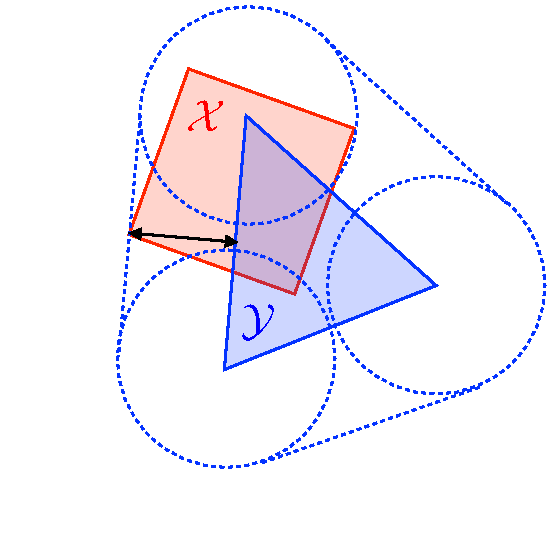
\includegraphics[width=.26\linewidth]{gromov-hausdorff/hausdorff-1}
\qquad
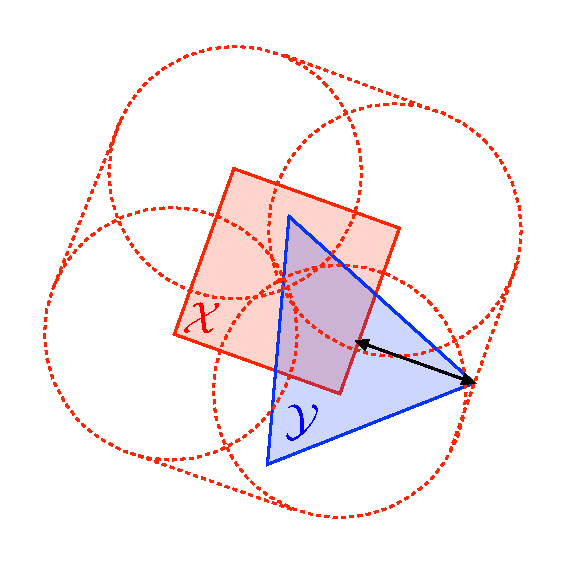
\includegraphics[width=.26\linewidth]{gromov-hausdorff/hausdorff-2}
\caption{\label{fig-hausdorff}
Computation of the Hausdorff distance in $\RR^2$. 
}
\end{figure}

Following~\citet{memoli-2011}, one remarks that this distance between sets $(A,B)$ can be defined similarly to the Wasserstein distance between measures (which should be somehow understood as ``weighted'' sets). One replaces the measures couplings~\eqref{eq-coupling-generic} by sets couplings
\eq{
	\Rr(A,B) \eqdef \enscond{ R \in \X \times \Y }{
	\begin{array}{l}
		\foralls a \in A, \exists b \in B, (a,b) \in R \\
		\foralls b \in B, \exists a \in A, (a,b) \in R
	\end{array}
	}.
}
With respect to Kantorovich problem~\eqref{eq-mk-generic}, one should replace integration (since one does not have access to measures) by maximization, and one has
\eql{\label{eq-hausf-couplings}
	\Hh_\Zz(A,B) = \uinf{ R \in \Rr(A,B) } \sup_{(a,b) \in R} d(a,b). 
}
%
Note that the support of a measure coupling $\pi \in \Couplings(\al,\be)$ is a set coupling between the supports, \ie $\Supp(\pi) \in \Rr( \Supp(\al),\Supp(\be) )$.
%
The Hausdorff distance is thus connected to the $\infty$-Wasserstein distance (see Remark~\ref{rem-p-inf}) and one has $\Hh(A,B) \leq \Wass_\infty(\al,\be)$ for any measure $(\al,\be)$ whose supports are $(A,B)$.


%%%%%%%%%%%%%%%%%%%%%%%%%%%%%%%%%%%%%%%%%%%%%%%%%%%%%%%%%%%%%%%%%%%%%%%%%%
\subsection{Gromov--Hausdorff distance}

The Gromov--Hausdorff (GH) distance~\citep{gromov-2001} (see also~\citep{edwards1975structure}) is a way to measure the distance between two metric spaces $(\X,d_\X), (\Y,d_\Y)$ by quantifying how far they are from being isometric to each other, see Figure~\ref{fig-gh}. It is defined as the minimum Hausdorff distance between every possible isometric embedding of the two spaces in a third one,
\eq{
	\Gg\Hh(d_\Xx,d_\Yy) \eqdef 
	\inf_{\Zz,f,g} \enscond{
		\Hh_\Zz(f(\Xx), g(\Yy))
	}{
		\begin{array}{l}
		f : \Xx \overset{\text{isom}}{\longrightarrow} \Zz\\
		g : \Yy \overset{\text{isom}}{\longrightarrow} \Zz
		\end{array}
	}.
}
Here, the constraint is that $f$ must be an isometric embedding, meaning that $d_\Zz(f(x),f(x'))=d_\Xx(x,x')$ for any $(x,x') \in \X^2$ (similarly for $g$). One can show that $\Gg\Hh$ defines a distance between compact metric spaces up to isometries, so that in particular $\Gg\Hh(d_\Xx,d_\Yy)=0$ if and only if there exists an isometry $h : \Xx \rightarrow \Yy$, \ie $h$ is bijective and $d_\Yy(h(x),h(x'))=d_\Xx(x,x')$ for any $(x,x') \in \Xx^2$. 

\begin{figure}[h!]
\centering
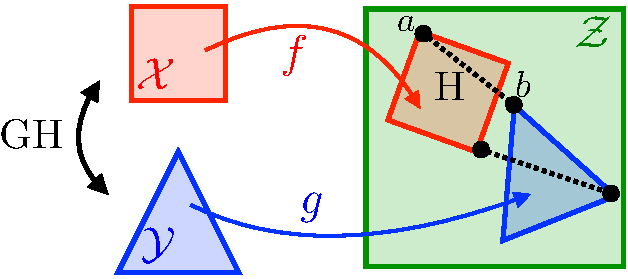
\includegraphics[width=.45\linewidth]{gromov-hausdorff/gh-concept}
\caption{\label{fig-gh}
The GH approach to compare two metric spaces.
}
\end{figure}

Similarly to~\eqref{eq-hausf-couplings} and as explained in~\citep{memoli-2011}, it is possible to rewrite equivalently the GH distance using couplings as follows:
\eq{
	\Gg\Hh(d_\Xx,d_\Yy) = \frac{1}{2} \uinf{ R \in \Rr(\X,\Y) } \sup_{ ((x,y),(x',y')) \in R^2 }
	|d_\Xx(x,x')-d_\Xx(y,y')|. 
}
For discrete spaces $\Xx = (x_i)_{i=1}^n, \Yy = (y_j)_{j=1}^m$ represented using a distance matrix $\distD = ( d_{\Xx}(x_i,x_{i'}) )_{i,i'} \in \RR^{n \times n}$,  $\distD' = ( d_{\Yy}(y_j,y_{j'}) )_{j,j'} \in \RR^{m \times m}$, one can rewrite this optimization using binary matrices $\VectMode{R} \in \{0,1\}^{n \times m}$ indicating the support of the set couplings $R$ as follows:
\eql{\label{eq-gh-coupling}
	\text{GH}(\distD,\distD') = \frac{1}{2} \uinf{ \VectMode{R} \ones >0,\VectMode{R}^\top \ones>0  } \max_{ (i,i',j,j') }
	\VectMode{R}_{i,j} \VectMode{R}_{j,j'} |\distD_{i,i'}-\distD_{j,j'}'|. 
}
The initial motivation of the GH distance is to define and study limits of metric spaces, as illustrated in Figure~\ref{fig-gh-limit}, and we refer to~\citep{burago2001course} for details. 
%
There is an explicit description of the geodesics for the GH distance~\citep{chowdhury2016constructing}, which is very similar to the one in Gromov--Wasserstein spaces, detailed in Remark~\ref{rem-geod-gw}. 

\begin{figure}[h!]
\centering
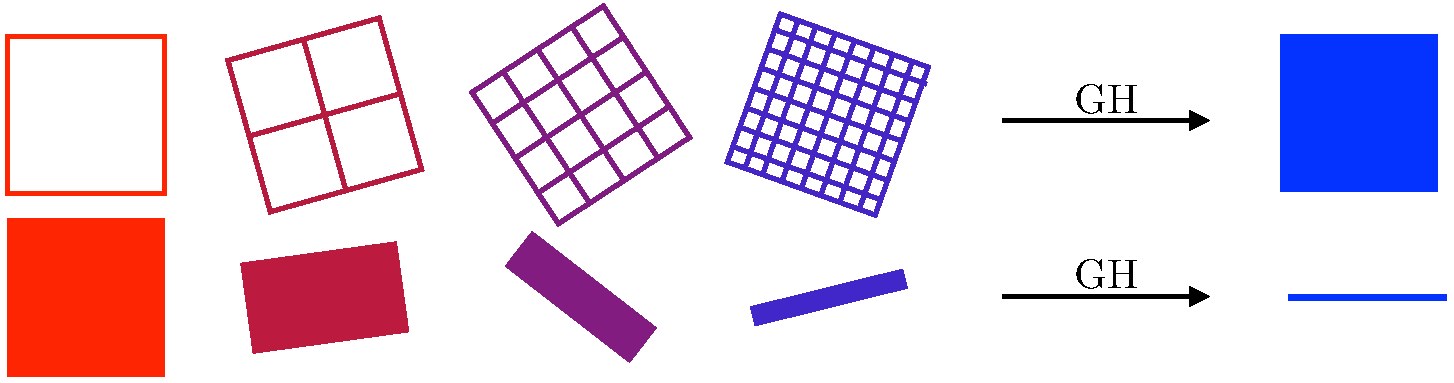
\includegraphics[width=1\linewidth]{gromov-hausdorff/gh-convergence}
\caption{\label{fig-gh-limit}
GH limit of sequences of metric spaces.  
}
\end{figure}

The underlying optimization problem~\eqref{eq-gh-coupling} is highly nonconvex, and computing the global minimum is untractable. It has been approached numerically using approximation schemes and has found applications in vision and graphics for shape matching~\citep{memoli2005theoretical,bronstein2006generalized}.

It is often desirable to ``smooth'' the definition of the Hausdorff distance by replacing the maximization by an integration. This in turn necessitates the introduction of measures, and it is one of the motivations for the definition of the GW distance in the next section.
 
%%%%%%%%%%%%%%%%%%%%%%%%%%%%%%%%%%%%%%%%%%%%%%%%%%%%%%%%%%%%%%%%%%%%%%%%%%
\subsection{Gromov--Wasserstein Distance}

Optimal transport needs a ground cost $\C$ to compare histograms $(\a,\b)$ and thus cannot be used if the bins of those histograms are not defined on the same underlying space, or if one cannot preregister these spaces to define a ground cost between any pair of bins in the first and second histograms, respectively. 
%
To address this limitation, one can instead only assume a weaker assumption, namely that two matrices $\distD \in \RR^{n \times n}$ and $\distD' \in \RR^{m \times m}$ quantify similarity relationships between the points on which the histograms are defined. A typical scenario is when these matrices are (power of) distance matrices.
%
The GW problem reads
\eql{\label{eq-gw-def}
	\GWD( (\a,\distD), (\b,\distD') )^2 \eqdef \umin{ \P \in \CouplingsD(\a,\b) } 
		\Ee_{\distD,\distD'}(\P)
}
\eq{
	\qwhereq
	\Ee_{\distD,\distD'}(\P) \eqdef 
		\sum_{i,j,i',j'} |\distD_{i,i'} - \distD'_{j,j'}|^2 \P_{i,j}\P_{i',j'},  
}
see Figure~\ref{fig-gw}.
%
This problem is similar to the GH problem~\eqref{eq-gh-coupling} when replacing maximization by a sum and set couplings by measure couplings.
%
This is a nonconvex problem, which can be recast as a quadratic assignment problem~\citep{loiola-2007} and is in full generality NP-hard to solve for arbitrary inputs. 
%
It is in fact equivalent to a graph matching problem~\citep{lyzinski-2015} for a particular cost.\todoK{detail QAP/graph matching}



\begin{figure}[h!]
\centering
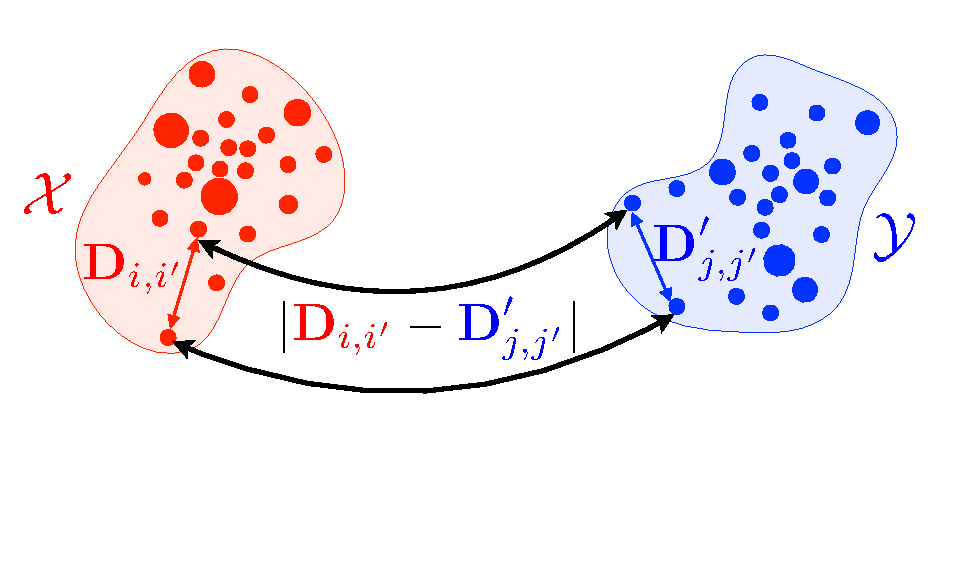
\includegraphics[width=.7\linewidth]{gw/gw-concept}
\caption{\label{fig-gw}
The GW approach to comparing two metric measure spaces.  
}
\end{figure}

One can show that $\GWD$ satisfies the triangular inequality, and in fact it defines a distance between metric spaces equipped with a probability distribution, here assumed to be discrete in definition~\eqref{eq-gw-def}, up to isometries preserving the measures.
%
This distance was introduced and studied in detail by~\citet{memoli-2011}. An in-depth mathematical exposition (in particular, its geodesic structure and gradient flows) is given in~\citep{SturmGW}. See also~\citep{schmitzer2013modelling} for applications in computer vision.
%
This distance is also tightly connected with the GH distance~\citep{gromov-2001} between metric spaces, which have been used for shape matching~\citep{memoli-2007,bronstein-2010}. 



%%%%%%%%%%%%%%%%%%%%%
\begin{rem2}{Gromov--Wasserstein distance}
	The general setting corresponds to computing couplings between metric measure spaces $(\X,\dist_\X,\al_\X)$
	and $(\Y,\dist_\Y,\al_\Y)$, where $(\dist_\X,\dist_\Y)$ are distances, while $\al_\X$ and $\al_\Y$ are measures on their respective spaces.
	%
	One defines 
	\begin{equation}
		\label{eq-gw-generic}
		\begin{split}
		&\GW( (\al_\X,\dist_\X), (\al_\Y,\dist_\Y) )^2 \eqdef \\
		&\umin{ \pi \in \Couplings(\al_\X,\al_\Y) } 
		\int_{\X^2 \times \Y^2}
		| \dist_\X(x,x')-\dist_\Y(y,y') |^2
		\d\pi(x,y)\d\pi(x',y').
		\end{split}
	\end{equation}
	$\GW$ defines a distance between metric measure spaces up to isometries, where one says that $(\X,\al_\X,\dist_\X)$ and $(\Y,\al_\Y,\dist_\Y) $ are isometric if there exists a bijection $\phi : \X \rightarrow \Y$ such that $\phi_{\sharp}\al_\X=\al_\Y$ and $\dist_\Y(\phi(x),\phi(x'))=\dist_\X(x,x')$.
\end{rem2}
%%%%%%%%%%%%%%%%%%%%%



%%%%%%%%%%%%%%%%%%%%%
\begin{rem2}{Gromov--Wasserstein geodesics}\label{rem-geod-gw}
The space of metric spaces (up to isometries) endowed with this $\GW$ distance~\eqref{eq-gw-generic} has a geodesic structure. \citet{SturmGW} shows that the geodesic between  $(\X_0,\dist_{\X_0},\al_0)$ and $(\X_1,\dist_{\X_1},\al_1)$ can be chosen to be 
$t \in [0,1] \mapsto (\X_0 \times \X_1,\dist_t,\pi^\star),$ where $\pi^\star$ is a solution of~\eqref{eq-gw-generic} and for all $((x_0,x_1), (x_0',x_1')) \in (\X_0 \times \X_1)^2$, 
\eq{
	\dist_t((x_0,x_1), (x_0',x_1')) \eqdef
	(1-t)\dist_{\X_0}(x_0,x_0') + t\dist_{\X_1}(x_1,x_1').
}
This formula allows one to define and analyze gradient flows which minimize functionals involving metric spaces; see~\citet{SturmGW}. It is, however, difficult to handle numerically, because it involves computations over the product space $\X_0 \times \X_1$. 
%
A heuristic approach is used in~\citep{peyre2016gromov} to define geodesics and barycenters of metric measure spaces while imposing the cardinality of the involved spaces and making use of the entropic smoothing~\eqref{eq-gw-entropy} detailed below.
\end{rem2}
%%%%%%%%%%%%%%%%%%%%%


%%%%%%%%%%%%%%%%%%%%%%%%%%%%%%%%%%%%%%%%%%%%%%%%%%%%%%%%%%%%%%%%%%%%%%%%%%
\subsection{Entropic Regularization}

To approximate the computation of $\GWD$, and to help convergence of minimization schemes to better minima, one can consider the entropic regularized variant
\eql{\label{eq-gw-entropy}
	\umin{ \P \in \CouplingsD(\a,\b) } 
		\Ee_{\distD,\distD'}(\P) - \varepsilon \HD(\P).
}
As proposed initially in~\citep{gold-1996,rangarajan-1999}, and later revisited in~\citep{2016-solomon-gw} for applications in graphics, one can use iteratively Sinkhorn's algorithm to progressively compute a stationary point of~\eqref{eq-gw-entropy}. 
%
Indeed, successive linearizations of the objective function lead to consider the succession of updates
\eql{\label{eq-gw-sinkh}
	\itt{\P} \eqdef \umin{ \P \in \CouplingsD(\a,\b) } \dotp{\P}{\it{\C}} - \varepsilon\H(\P)
		\qwhereq
}
\eq{
		\it{\C} \eqdef \nabla \Ee_{\distD,\distD'}(\it{\P}) = -\distD \it{\P} \distD', 
}
which can be interpreted as a mirror-descent scheme~\citep{2016-solomon-gw}. Each update can thus be solved using Sinkhorn iterations~\eqref{eq-sinkhorn} with cost $\it{\C}$.
%
Figure~\ref{fig-gw-iter} displays the evolution of the algorithm. 
%
Figure~\ref{fig-gw-sinkhorn} illustrates the use of this entropic GW to compute soft maps between domains. 


\newcommand{\FigGW}[1]{\includegraphics[width=.21\linewidth]{gromov-wasserstein/#1}}

\begin{figure}[h!]
\centering
\begin{tabular}{@{}c@{\hspace{2mm}}c@{\hspace{2mm}}c@{\hspace{2mm}}c@{}}
\imgBox{\FigGW{coupling-1}}&
\imgBox{\FigGW{coupling-2}}&
\imgBox{\FigGW{coupling-3}}&
\imgBox{\FigGW{coupling-4}}\\
\FigGW{matching-1}&\FigGW{matching-2}&\FigGW{matching-3}&\FigGW{matching-4}\\
$\ell=1$ & $\ell=2$ & $\ell=3$ & $\ell=4$ 
\end{tabular}
\caption{\label{fig-gw-iter}
Iterations of the entropic GW algorithm~\eqref{eq-gw-sinkh} between two shapes $(x_i)_i$ and $(y_j)_j$ in $\RR^2$, initialized with $\P^{(0)}=\a \otimes \b$. The distance matrices are $\distD_{i,i'} = \norm{x_i-x_{i'}}$ and $\distD_{j,j'}' = \norm{y_j-y_{j'}}$. 
%
Top row: coupling $\it{\P}$ displayed as a 2-D image.
%
Bottom row: matching induced by $\it{\P}$ (each point $x_i$ is connected to the three $y_j$ with the three largest values among $\{\it{\P}_{i,j}\}_j$). The shapes have the same size, but for display purposes, the inner shape $(x_i)_i$ has been reduced.
}
\end{figure}



\begin{figure}[h!]
\centering
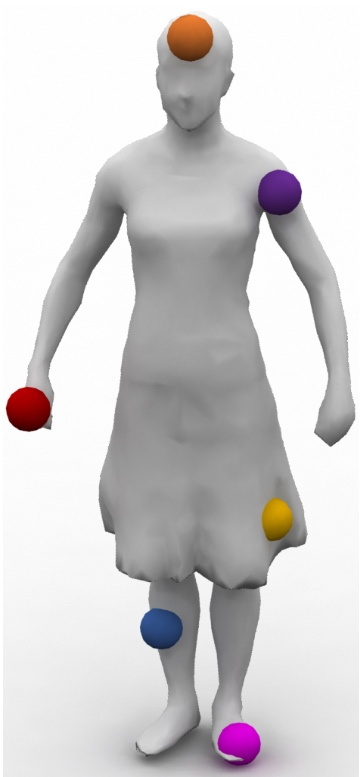
\includegraphics[height=.27\linewidth]{gw/source}
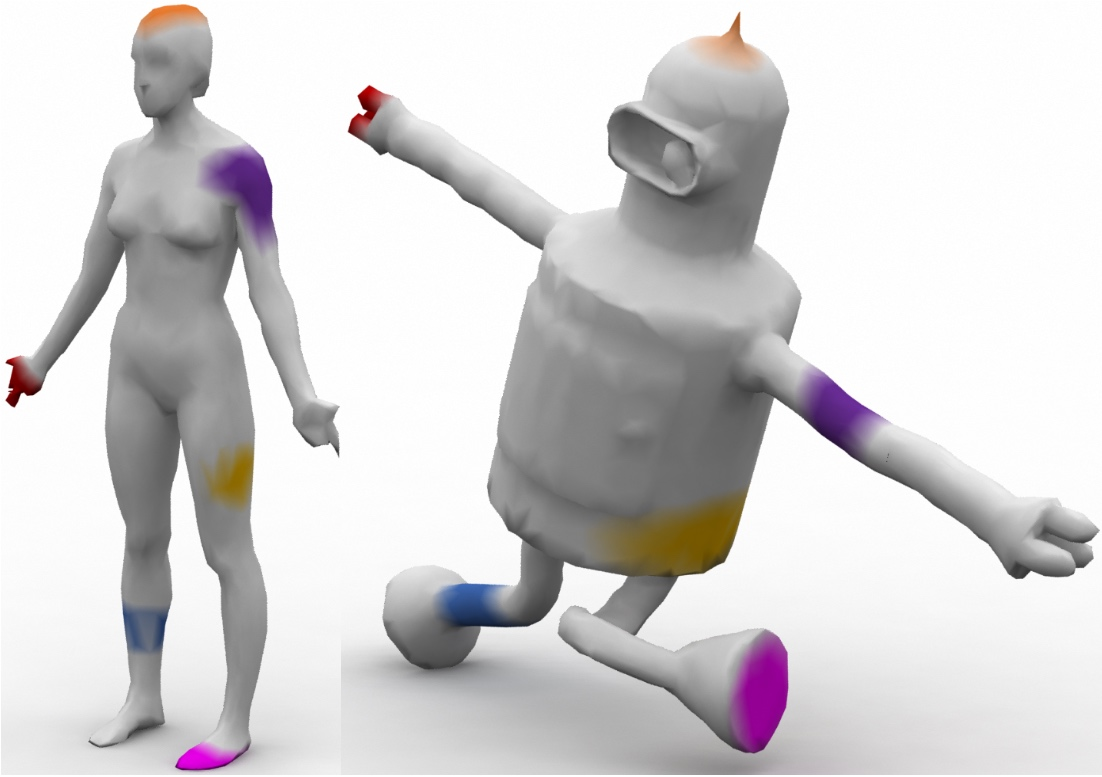
\includegraphics[height=.27\linewidth]{gw/target-surf}
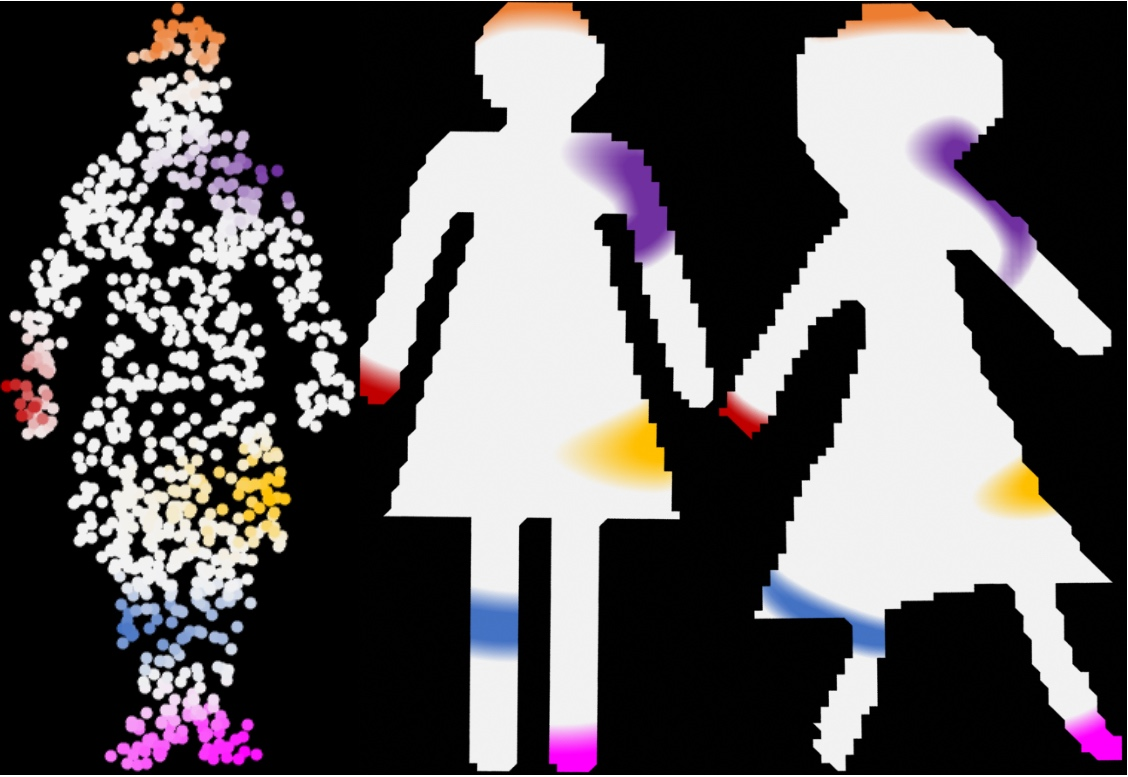
\includegraphics[height=.27\linewidth]{gw/target-2d}
\caption{\label{fig-gw-sinkhorn}
Example of fuzzy correspondences computed by solving GW problem~\eqref{eq-gw-entropy} with Sinkhorn iterations~\eqref{eq-gw-sinkh}. Extracted from~\citep{2016-solomon-gw}.
}
\end{figure}



